% Three lines at \Huge on this measure -- "Chygraph representation" is a
% shade too wide for one. Broken by hand so the last line is a phrase rather
% than an orphaned "systems"; the optional argument keeps the contents and
% the running head on one line.
\chapter[Chygraph representation of real systems]{Chygraph\\representation\\of real systems}
\label{ch:data}

Chapter~\ref{ch:chygraphs} defined an object. In this chapter we ask where to
get hold of it. Everything measured here is new; the
worked example of a publication as a complex is Chapter~\ref{ch:chygraphs}'s,
and drawn rather than measured. There are exactly two routes, they behave very differently, and
which of the two applies decides in advance how well the theory of the next ten
chapters will work on the data, so it comes before the theory rather than
after.

The first route is the easy one. Some systems record their groups. A paper
lists its authors, a purification recovers a set of proteins together, a
reaction names its substrates, a work package names its predecessors. Where the
groups are in the data, the chygraph is read straight off them, and the only
decisions are which layers to use.

The second route is the one most people are on. There is a graph, and nothing
else --- a list of pairs, with whatever produced them long since discarded. Then
the complexes have to be \emph{found}, and the natural candidates are the dense
motifs: the maximal cliques. This route works, but it works to a degree that
varies enormously from one network to another, and Sec.~\ref{sec:promoting}
measures how much on ten real networks.

There is also a third thing one does, which is not a route into real data at
all but is needed throughout the book: generating random chygraphs to check the
theory against. That is Sec.~\ref{sec:sampling}.

\begin{figure}[t]
\centering
\begin{adjustbox}{max width=\linewidth}
\begin{tikzpicture}
% ---------------- route 1: the groups are in the data
\begin{scope}
  \node[tb,anchor=west] at (-0.2,3.15) {(a) the groups are in the data};
  \node[lb,anchor=west,align=left] at (-0.2,2.55)
    {a paper and its authors,\\ a purification, a reaction};
  \node[nd] (s1) at (0.30,1.55) {}; \node[nd] (s2) at (1.10,1.85) {};
  \node[nd] (s3) at (1.05,1.05) {}; \node[nd] (s4) at (2.10,1.45) {};
  \begin{scope}[on background layer]
    \node[cx,fill=black!26,fill opacity=0.7,fit=(s1)(s2)(s3)]{};
    \node[cx,fill=black!26,fill opacity=0.7,inner sep=3.8pt,fit=(s3)(s4)]{};
  \end{scope}
  \draw[msg] (1.05,0.65) -- (1.05,0.10);
  \node[lb,anchor=west,align=left] at (-0.2,-0.42)
    {write the layers down:\\ the complexes are given};
\end{scope}
% ---------------- route 2: only a graph
\begin{scope}[xshift=6.0cm]
  \node[tb,anchor=west] at (-0.2,3.15) {(b) only a graph survives};
  \node[lb,anchor=west,align=left] at (-0.2,2.55)
    {an interactome, a power grid,\\ a road network};
  \node[nd] (t1) at (0.30,1.55) {}; \node[nd] (t2) at (1.10,1.85) {};
  \node[nd] (t3) at (1.05,1.05) {}; \node[nd] (t4) at (2.10,1.45) {};
  \draw[lnk] (t1)--(t2)--(t3)--(t1) (t3)--(t4);
  \draw[msg] (1.05,0.65) -- (1.05,0.10);
  \node[lb,anchor=west,align=left] at (-0.2,-0.42)
    {find the complexes:\\ promote the maximal cliques};
\end{scope}
\end{tikzpicture}
\end{adjustbox}
\caption{\textbf{Two routes in.} (a) When the data records its groups, the
complexes are given and the modelling is a choice of layers. (b) When only a
list of pairs survives, the complexes must be found, and the maximal cliques are
the natural candidates. Route (b) is a reconstruction and can fail;
Sec.~\ref{sec:promoting} measures how badly, and finds that the worst case is a
network that was on route (a) before somebody flattened it.}
\label{fig:tworoutes}
\end{figure}

\section{Systems whose interactions are not pairwise}
\label{sec:systems}

Four families of system, chosen because between them they cover most of what
anybody wants to do with this construction, and because they differ in exactly
the way that matters --- how much of the group structure survives into the file
that is finally distributed.

\paragraph{Papers and their authors.} Treated at length in
Sec.~\ref{sec:paper}. Atoms are authors, complexes are publications, the
interior hypergraph of a publication has two hyperedges --- author list and
reference list --- and a citation is a complex included in a complex. Of the
four families this is the only one that genuinely needs the interior to be a
hypergraph rather than a flat set, and it is the one that needs inclusion to
recurse. It is the reason the definition is what it is.

\paragraph{Proteins in complexes.} A protein complex is a set of proteins that
act as a unit --- the ribosome, the proteasome, a transcription factor assembly.
Affinity purification recovers such a set in one experiment: a bait protein is
pulled down and everything bound to it comes with it. That is group-level data
in the most literal sense, and the natural chygraph has proteins as atoms and
purifications as complexes, with one layer per experiment type. Two-hybrid
screening, by contrast, tests one pair at a time and produces genuinely pairwise
data. The two kinds of experiment therefore produce different objects, and
Sec.~\ref{sec:promoting} shows they behave completely differently under
promotion.

\paragraph{Reactions and their species.} A chemical reaction consumes some
species and produces others, and the natural complex has an interior with two
hyperedges --- substrates and products --- exactly like a publication's authors
and references. Metabolic networks are routinely drawn as graphs of species
joined when a reaction connects them, which loses the stoichiometry, the
direction and the grouping in one move.

\paragraph{Activities and their dependencies.} A project schedule is a set of
activities and the logical constraints between them, and constraints are often
group-level: an activity may start when \emph{all} of a set of predecessors have
finished, or when \emph{any} one has. Those are two different interiors on the
same complex --- a distinction Chapter~\ref{ch:giant} makes precise as AND-logic
against OR-logic, and one that no pairwise graph can carry.

Table~\ref{tab:systems} collects the four, together with what the pairwise
graph keeps of each and what it throws away.

\begin{table}[t]
\centering\small
\begin{tabular}{lll}
\hline\hline
system & atoms & complexes\\
\hline
literature & authors & publications (authors $+$ references)\\
proteomics & proteins & purifications, or screened pairs\\
metabolism & species & reactions (substrates $+$ products)\\
projects & activities & dependency sets (AND or OR)\\
\hline\hline
\end{tabular}
\caption{\textbf{Four systems, one construction.} In each case the complexes are
what the experiment or the record actually produces, and the pairwise graph is
what is left after the grouping has been thrown away.}
\label{tab:systems}
\end{table}

\section{Reading the layers off group data}
\label{sec:layers-data}
\index{group data}

When the groups are given, building the chygraph is bookkeeping, and there are
three decisions to make.

\emph{What is an atom.} Whatever the modelling declines to decompose further.
This is a
modelling choice and it should be made once, explicitly, because everything
downstream inherits it.

\emph{What the layers are.} One layer per statistically distinct kind of
complex. Distinctness is the operative word: two kinds of complex belong in
different layers when their chy-degree distributions or cardinality
distributions differ, and in the same layer when they do not. Two-hybrid
interactions and affinity purifications are different layers. Author lists and
reference lists are different layers. A hypergraph with a broad spread of
cardinalities takes one layer per cardinality, which sounds extravagant and is
not, because $L$ enters the theory only as the size of an $L\times L$
determinant.

\emph{Whether the layers are independent.} The theory of
Chapters~\ref{ch:percolation} and~\ref{ch:statmech} assumes that a complex's
participation in one layer says nothing about its participation in another,
so that the generating functions factorise. That is often false in data --- a
protein in many purifications is usually also in many two-hybrid pairs --- and
the repair is to replace the marginals by a joint $\Phi$, with the
unconditional first moments replaced by inclusion-biased second moments.
Chapter~\ref{ch:giant} does that in general and shows it matters: two ensembles
with \emph{identical} marginals can have different thresholds. So this decision
is not cosmetic, and the way to make it is to measure the correlation between
layer memberships before assuming it away.

One rule of thumb, with the evidence for it in Sec.~\ref{sec:promoting}:
\textbf{where the group data exists, use it; do not flatten it to a graph and
then try to recover the groups.} The flattening is not invertible, and what
comes back is worse than either the graph or the groups.

\section{Promoting the cliques of a real graph}
\label{sec:promoting}
\index{clique promotion|textbf}
\index{configuration model}
\index{clustering!manufactured by a null model}

On the other route a graph is given and a chygraph has to be built from it. The
recipe of
Sec.~\ref{sec:everything} says to promote the dense motifs, and with no
information about which motifs are meaningful, the maximal cliques are the
default choice: a maximal clique is a set of nodes all of which are joined, not
contained in any larger such set, and every edge lies in at least one.

Two questions decide whether this works, and both are measurable before any
physics is done.

The first is whether the resulting ensemble has finite moments. The threshold
tensor of Chapter~\ref{ch:percolation} needs the excess cardinality seen from a
member,
\begin{equation}
  \bar s=\frac{\ave{c^{2}}}{\ave{c}}-1,
  \label{eq:sbar-data}
\end{equation}
to be finite --- which is to say, the clique-size distribution needs a converged
second moment. The reference value is easy to remember: a graph with no
clustering at all has almost every edge in a maximal clique of size two, and
sits at $\bar s\approx1$.

The second is whether the cliques overlap. Section~\ref{sec:treelike} established
that a chygraph is treelike only when its complexes meet in at most one atom, so
the diagnostic is the fraction of intersecting clique pairs that share two or
more atoms. Call it $\mathrm{shared}_{2+}$. It is zero for a treelike chygraph
and one for a family in which every intersection is an edge or larger.

Table~\ref{tab:real} and Figure~\ref{fig:realoverlap} report both for ten real
networks --- eight protein interaction datasets, a power grid and a road network
--- each carried alongside its degree-matched configuration model, which
rewires everything at fixed degree sequence. (Whether that destroys the
clustering, which is what one usually assumes it does, turns out to be the third
finding below.)

\begin{table}[t]
\centering\small
\begin{tabular}{lrrrrrr}
\hline\hline
 & & & \multicolumn{2}{c}{$\bar s$} & \multicolumn{2}{c}{shared$_{2+}$}\\
network & $\ave{k}$ & $C$ & real & ctrl & real & ctrl\\
\hline
Collins yeast & 16.57 & 0.648 & 21.91 & 1.97 & 0.903 & 0.055\\
Yeast (Y2H) & 2.67 & 0.071 & 1.15 & 1.02 & 0.014 & 0.001\\
Human (Vidal) & 4.32 & 0.072 & 1.26 & 1.09 & 0.022 & 0.007\\
Human (Stelzl) & 3.85 & 0.006 & 1.05 & 1.21 & 0.003 & 0.022\\
Human (Figeys) & 5.79 & 0.040 & 1.21 & 2.37 & 0.022 & 0.155\\
PDZ domains & 2.60 & 0.007 & 1.01 & 1.10 & 0.000 & 0.015\\
C. elegans WI8 & 3.20 & 0.022 & 1.13 & 1.11 & 0.014 & 0.012\\
C. elegans 2007 & 2.71 & 0.017 & 1.09 & 1.12 & 0.010 & 0.014\\
Power grid & 2.67 & 0.080 & 1.14 & 1.00 & 0.016 & 0.000\\
Euroroad & 2.51 & 0.019 & 1.04 & 1.00 & 0.001 & 0.000\\
\hline\hline
\end{tabular}

\caption{\textbf{The chygraph a real graph has.} Maximal cliques promoted to
complexes, for ten networks and for their degree-matched configuration models
(``ctrl'', mean of three realisations). $C$ is the average clustering
coefficient, $\bar s$ the excess cardinality of Eq.~\eqref{eq:sbar-data}, and
$\mathrm{shared}_{2+}$ the fraction of intersecting complex pairs sharing two or
more atoms --- the pairs the construction cannot represent. Generated by
\code{figs/real\_chygraphs.py}.}
\label{tab:real}
\end{table}

\begin{figure}[t]
\centering
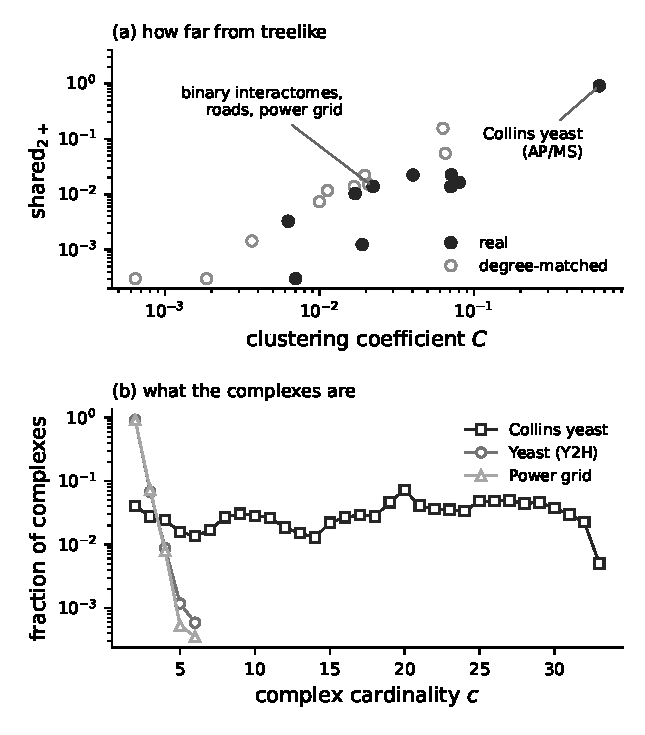
\includegraphics[width=0.86\linewidth]{figs/fig-real-overlap.pdf}
\caption{\textbf{How far from treelike, and why.} (a) Overlap against clustering
for the ten networks of Table~\ref{tab:real}, filled for the real network and
open for its degree-matched control. (b) The cardinality distribution of the
promoted complexes. Two-hybrid interactomes and infrastructure networks are
almost entirely complexes of cardinality two with a thin tail; the
purification-derived network is a different object altogether, with complexes
out to cardinality $33$ and no characteristic size.}
\label{fig:realoverlap}
\end{figure}

Three findings follow, and the third is the least expected.

\paragraph{Most real graphs promote almost perfectly.} The two-hybrid
interactomes, the power grid and the road network all sit at $\bar s$ between
$1.01$ and $1.26$ --- within about a quarter of the clustering-free reference
--- and at $\mathrm{shared}_{2+}$ between $0.000$ and $0.022$. Fewer than one
intersecting clique pair in forty-four shares an edge. For these networks the
chygraph of maximal cliques is treelike for practical purposes, and the theory
of the next ten chapters applies to them essentially without correction. The
obstruction Chapter~\ref{ch:overlap} is about is therefore specific rather than
generic, and one can tell in advance whether one has it.

\paragraph{One network fails completely.} The
Collins yeast dataset sits at $\bar s=21.9$ against a control of $1.97$, at
$\mathrm{shared}_{2+}=0.903$, and its average edge is covered by $114$ distinct
maximal cliques. Nine intersecting clique pairs in ten share an edge or more.
Promotion has failed categorically.

Collins \emph{et al.} measured
co-complex associations by affinity purification and mass spectrometry: a
purification recovers a group of proteins together, and the public network
records that group by joining all pairs within it. The graph is a union of
cliques, one per purification, and it is a union of \emph{overlapping} cliques
because proteins belong to several complexes. So the dataset was on route (a) of
Figure~\ref{fig:tworoutes}, and somebody flattened it onto route (b). Trying to
recover the groups by clique promotion is an attempt to invert that flattening,
and Figure~\ref{fig:realoverlap}b shows what comes back: a cardinality
distribution running to $33$ with no characteristic size, because the maximal
cliques of a union of overlapping cliques are not the original groups but every
combination the overlaps permit.

That is the rule of Sec.~\ref{sec:layers-data} arriving as a measurement. The
underlying purifications would have made a perfectly good chygraph with a
handful of layers and modest cardinalities. The flattened graph does not, and no
amount of care in the promotion step will repair it, because the information was
destroyed before the file was written.

\paragraph{The control is not always the cleaner object.} Destroying the
clustering might be expected only to reduce the overlap, so that the
configuration model would always sit below the real network in
Figure~\ref{fig:realoverlap}a. In four of the ten it sits \emph{above}. For the
Figeys human interactome the control's $\mathrm{shared}_{2+}$ is $0.155$ against
the real network's $0.022$, a factor of seven the wrong way, and its $\bar s$ is
$2.37$ against $1.21$.

The mechanism is degree heterogeneity. A configuration model with a heavy tail
gives its hubs so many neighbours that some of those neighbours are shared by
chance, and shared neighbours are triangles, and triangles are cliques of
cardinality three. So the control does not have zero clustering; it has however
much its degree sequence manufactures, and that quantity grows with the degree
heterogeneity $\ave{k^{2}}/\ave{k}$. The Figeys network is the most heterogeneous of
the ten by a wide margin --- $\ave{k^{2}}/\ave{k}=56$, half again the next
largest and four times the median --- and it is the one whose control overlaps
most, at $0.155$.

Which of the two wins is then a race between the clustering a network really has
and the clustering its degree sequence would manufacture anyway. The control
wins on Stelzl ($C=0.006$), PDZ ($C=0.007$), Figeys ($C=0.040$) and, narrowly,
the 2007 \emph{C. elegans} screen ($C=0.017$, $0.014$ against $0.010$): all
networks with little real clustering and enough heterogeneity to manufacture
some. It loses on Euroroad, which has almost no clustering either ($C=0.019$)
but a light tail --- $\ave{k^{2}}/\ave{k}=3.1$, the lowest here --- so its
control manufactures nothing at all and returns $\mathrm{shared}_{2+}=0.000$.
And it loses on every network with real clustering to spare, Vidal and the power
grid among them.

The practical consequence is a caution rather than a result, and it applies to
every degree-matched comparison in this book, including the ones in
Chapter~\ref{ch:cover} that the whole programme rests on. \emph{Degree-matched}
does not mean \emph{unclustered}. On a heavy-tailed degree sequence the null
model manufactures clustering, and a comparison that reads a difference between
network and control as ``the effect of clustering'' is only valid once one has
checked how much clustering the control has. Section~\ref{sec:hrg-data} is careful
about this for exactly this reason.

\section{Hyperbolic random graphs}
\label{sec:hrg-data}
\index{hyperbolic random graph|textbf}

The real networks of Table~\ref{tab:real} have one drawback as a test bed: their
clustering is whatever it is, and cannot be turned. For the quantitative work of
Chapters~\ref{ch:cover} and~\ref{ch:overlap} the book leans instead on a
synthetic ensemble in which it can be --- hyperbolic random graphs, which place
nodes in a disc of hyperbolic geometry and join those that are close. They have
three properties that together make them the right instrument: a power-law
degree distribution with a tunable exponent $\tau$, strong clustering that comes
from the geometry rather than being inserted by hand, and a degree-matched
configuration model available as a control that has the same $P(k)$ and the same
assortativity to within a few per cent.

Whether a chygraph can be built on them at all is the question of
Eq.~\eqref{eq:sbar-data} again, and it has a sharp answer.

\begin{table}[t]
\centering\small
\begin{tabular}{lcccc}
\hline\hline
$\tau$ & $\theta$ (HRG) & $\theta$ (ctrl) & ratio & $\theta$ (ratio)\\
\hline
$2.9$ & $0.000$--$0.001$ & $-0.03$--$0.00$ & $1.76$--$4.77$ & $+0.003$--$0.028$\\
$2.5$ & $0.009$--$0.024$ & $-0.00$--$0.01$ & $1.79$--$3.52$ & $+0.009$--$0.015$\\
$2.1$ & $0.28$--$0.40$ & $0.42$--$0.58$ & $\to1$ & $-0.12$--$-0.18$\\
\hline
$3.5$ & flat & flat & $2.87$--$4.89$ & flat\\
$4.5$ & flat & flat & $2.95$--$5.06$ & flat\\
\hline\hline
\end{tabular}
\caption{\textbf{When the clique ensemble exists.} Growth exponent $\theta$ of
the excess cardinality $\bar s$ with $n$, over $n=10^{3}$ to $3\times10^{5}$,
for hyperbolic random graphs and their degree-matched controls. Every entry is
an exponent; in the two light-tailed rows the control is not merely flat but
flat at the Erd\H{o}s--R\'enyi value, $\bar s\to1.00$. The paired ratio
is taken at identical degree sequence and seed, so $P(k)$ and assortativity are
held fixed and clustering is the only difference. The same letter serves the
core exponent of Chapter~\ref{ch:cover}, but in
Chapters~\ref{ch:percolation} and~\ref{ch:giant} $\theta$ is the threshold
determinant and $\beta$ the order parameter exponent, while in Part~III $\beta$
is the inverse temperature.}
\label{tab:ensemble}
\end{table}

For $\tau\ge2.5$ the second moment converges and the paired ratio is a converged
constant between $1.8$ and $4.8$. The clustering signal is a multiplicative
factor that does not wash out with size, which is what one needs: a finite-size
artefact would have shrunk. Erd\H{o}s--R\'enyi graphs, which have finite
$\ave{k^{2}}$ and no clustering, sit at $\bar s=0.937$, $0.996$ and $1.000$ for
mean degree $2$, $4$ and $8$, flat to three decimals from $n=10^{4}$ upward, and
the control above $\tau=3$ returns to that value. Those are the reference points
that make the ratio meaningful. They are computed counting an isolated vertex as
a complex of cardinality one, which is what drags the mean-degree-two figure
below one; Table~\ref{tab:real} works on a largest connected component, where
the question does not arise.

At $\tau=2.1$ it fails, and it fails in an instructive direction. Both the graph
and its control diverge, and \emph{the control diverges faster}, so the paired
ratio decays toward one. Nothing measured in that range separates clustering
from the tail --- which is the caution of Sec.~\ref{sec:promoting} again, now in
a synthetic setting where it can be traced to its cause. A heavy enough tail
manufactures cliques at hubs without any geometry at all, and when it does, the
control is no longer a control. This is why Chapter~\ref{ch:cover} treats
$\tau=2.1$ as uninformative rather than as a discrepancy to be explained, and
why the light-tailed rows of Table~\ref{tab:ensemble} have to be run at all:
only where $\ave{k^{2}}$ is finite does a geometry-free control provide a clean
baseline.

One check that the measurement is reading the right quantity. The largest
clique in a hyperbolic random graph should scale as $n^{(3-\tau)/2}$
\citep{friedrich2015}, which is $0.45$, $0.25$ and $0.05$ at $\tau=2.1$, $2.5$
and $2.9$. Measured, it is $n^{0.37}$, $n^{0.20}$ and $n^{0.07}$, averaged over
mean degrees $2$, $4$ and $8$: below theory in the two heavy-tailed rows, as one
expects at finite $n$, and above it in the third, where the predicted exponent
is smaller than the spread across mean degrees ($0.06$ to $0.09$) and the
comparison decides nothing. What the check establishes is the trend --- a
ninefold range in the predicted exponent tracked over a fivefold range in the
measured one --- and not the value of any one row.

\section{How much overlap, and what it buys}
\label{sec:overlap-data}
\index{overlap!between complexes}

The single number to take away from this chapter is $\mathrm{shared}_{2+}$,
because it is an advance warning. It costs a clique enumeration to compute, it
requires no theory at all, and it says how much of the answer the next ten
chapters can be expected to get.

At $\mathrm{shared}_{2+}\lesssim0.02$ --- nine of the ten networks of
Table~\ref{tab:real} --- the chygraph is treelike for practical purposes and the
theory should be quantitative. On hyperbolic random graphs, where the maximal
cliques share edges as a matter of course, it is not: there
Chapter~\ref{ch:overlap} measures the chygraph recovering between $77$ and $100$
per cent of the leaf-removal core, with the deficit largest at intermediate
density, where overlap is largest, and vanishing at both ends --- when the graph
is sparse enough that cliques rarely meet, and when it is dense enough that
almost everything is core anyway. And at $\mathrm{shared}_{2+}=0.9$, which is
the flattened purification data, one should not be running the theory at all;
one should be going back for the purifications.

\section{Sampling from an ensemble}
\label{sec:sampling}
\index{random chygraph}

The rest of the book needs a way of generating chygraphs to order, since every
analytical result in
Chapters~\ref{ch:percolation} to~\ref{ch:satisfiability} is checked against
simulation on a finite instance.

The construction is the chygraph version of the configuration model. Draw a
chy-degree for each atom from $\Phi$, layer by layer; draw a cardinality for
each complex from the corresponding distribution; then match the resulting stubs
at random within each layer. What comes out is a random chygraph with the
prescribed first-moment matrices $\ave{\kappa}$, $\ave{\kbar}$, $\ave{s}$ and
$\ave{\sbar}$ of Sec.~\ref{sec:ensembles} and no further structure --- in
particular, complexes meet in at most one atom with probability approaching one
as the chygraph grows, which is exactly the r\'egime the theory assumes.

That last clause is why simulation agreement is a weaker test than it looks. A random chygraph built this way
satisfies the treelike condition by construction, so a Monte Carlo check on it
tests the recursion and \emph{not} the assumption that the recursion rests on.
Testing the assumption needs an object whose complexes really do overlap, which
is what the hyperbolic random graphs of Sec.~\ref{sec:hrg-data} and the rewired
control of Chapter~\ref{ch:cover} are for. Both kinds of check appear throughout
the book and they answer different questions; the text says which is which at
each point.

\medskip

A closing note on what this chapter does not contain. Every empirical number in
it is measured on a \emph{graph} --- ten real ones and one synthetic family ---
and on the chygraphs recovered from them by promotion. None is measured on a
dataset that came with its groups intact. The publications chygraph of
Figure~\ref{fig:publications} is drawn and not measured; so are the reaction and
project constructions of Sec.~\ref{sec:systems}. Building those objects from
real records, measuring their layer structure and the correlations between
layers, and running the machinery of the following chapters on them, is the most
obvious piece of work this book leaves undone, and Sec.~\ref{sec:promoting} is
the argument for doing it: the one dataset here that began as
group data is the one where the graph representation fails hardest.
